\documentclass[10pt,a4paper]{article}
\usepackage[margin=24mm]{geometry}
\usepackage[T1]{fontenc}
\usepackage{lmodern,amsmath,amssymb,booktabs,graphicx,microtype}
\usepackage[hidelinks]{hyperref}
\setlength{\parskip}{4pt}
\setlength{\parindent}{0pt}
\newcommand{\R}{\mathbb{R}}
\title{ForceWindow: terminal load identifiability\\from finite displacement records}
\author{}
\date{}
\begin{document}
\maketitle
\vspace{-12mm}
\begin{abstract}
How much can an unloaded observation tail reveal about the end of an applied force?
This reproducible synthetic study combines an exact held-load oscillator map,
a C++ state-recursion adjoint, and Python ridge inversion. With observations
taken at the starts of the force intervals, the final force coefficient is
in an exact nullspace. Extending the record removes this causal obstruction,
but does not guarantee smaller error for a fixed force and regularization.
For the specified 120-interval example, expected force RMSE is 0.04264 N with
no tail, 0.04556 N with one additional sample, and 0.03936 N with 80 additional
samples. These are analytical noise expectations for one prescribed load,
not measured experimental performance. Independent SVD inversion and an
analytical step response check the discrete implementation. A separate
smooth-input refinement study identifies second-order displacement error
from approximating the forcing, despite exact propagation of each held load.
\end{abstract}

\section{Question, scope, and mechanics}
Force identification from measured motion is sensitive both to noise and to
the interval of observation. We ask whether a known unloaded tail improves
identification of late forces, and how to distinguish an unobservable
coefficient from a numerically inaccurate solver. The study is an original
educational implementation, not a claim of a new inversion algorithm.
Its conceptual provenance is discrete-time state-space and convolution
material inspected in DTU MLSP, chapter 3. No private course content or
experimental datasets are distributed.

We assume a known linear single-degree-of-freedom system initially at rest:
\begin{equation}
 m\ddot q+c\dot q+kq=f(t),\qquad q(0)=\dot q(0)=0.
 \label{eq:mechanics}
\end{equation}
Mass $m>0$, damping $c\geq0$, and stiffness $k\geq0$ are constants.
The input has $N$ independent constant values $f_j$ on
$[j\Delta t,(j+1)\Delta t)$ and is exactly zero after $N\Delta t$.
Displacement is sampled at $t_i=i\Delta t$, $i=0,\ldots,N+L-1$,
where $L\geq0$ is the observation-tail count. Thus $L=0$ ends at
$(N-1)\Delta t$; $L=1$ includes the end of the final load interval.
Sensors have independent, zero-mean errors of common standard deviation
$\sigma$, without timing error. Unknown initial conditions, sensor filtering,
parameter uncertainty, and unrecorded subsequent loading are excluded.

Let $x=(q,\dot q)^T$, $C=(1,0)$, and
\begin{equation}
 F=\begin{pmatrix}0&1\\-k/m&-c/m\end{pmatrix},\quad
 g=\begin{pmatrix}0\\1/m\end{pmatrix},\qquad
 \exp\!\left[\Delta t\begin{pmatrix}F&g\\0&0\end{pmatrix}\right]
 =\begin{pmatrix}A&b\\0&1\end{pmatrix}.
 \label{eq:exponential}
\end{equation}
This block exponential avoids an inverse of $F$, including for a free mass.
It gives the exact zero-order-hold transition up to floating-point error
\cite{scipyZOH}. It does not make arbitrary continuous forces exactly constant.

\newpage
\section{Operator, adjoint, and regularized inversion}
The zero-state prediction is $x_{i+1}=Ax_i+b f_i$, $y_i=Cx_i$, with
$f_i=0$ for $i\geq N$. Hence the matrix $H\in\R^{(N+L)\times N}$ has entries
\begin{equation}
 H_{ij}=\begin{cases}CA^{i-j-1}b,&i>j,\\0,&i\leq j.\end{cases}
 \label{eq:H}
\end{equation}
When $L=0$, $He_{N-1}=0$ exactly. No improvement in precision or optimization
can identify that coefficient from these data. For $L=1$ and $Cb\neq0$,
the last $N$ rows are triangular with nonzero diagonal; they have full rank.
Full rank alone says little about noise amplification. Particular sampling
intervals can also lose information, so full rank is not assumed universally.

The C++ forward pass stores two state coordinates and the output vector.
Its Euclidean transpose action uses $p_{N+L}=0$ and a reverse sweep:
\begin{equation}
 (H^Tr)_i=b^Tp_{i+1}\quad(i<N),\qquad
 p_i=A^Tp_{i+1}+C^Tr_i.
 \label{eq:adjoint}
\end{equation}
The gradient is recorded before adding $r_i$. Reversing this order would
silently change the observation timing. Each operator action costs
$O(N+L)$ arithmetic and linear input/output storage, with constant auxiliary
state storage. Python-to-C++ list conversions also cost linear time and
memory. No performance speedup is claimed here.

We solve the strictly convex ridge problem
\begin{equation}
 \widehat f=\arg\min_f\{\|Hf-y\|_2^2+\lambda^2\|f\|_2^2\},
 \qquad\lambda>0,
 \label{eq:ridge}
\end{equation}
with SciPy LSQR and the C++ forward/transpose routines \cite{paige,scipyLSQR}.
In SI units $\lambda$ has units m/N. It is a user-supplied regularization
scale, not a force smoothness penalty or a noise standard deviation. LSQR
uses $\mathtt{atol}=\mathtt{btol}=10^{-11}$, a limit of $10N$ iterations,
and condition limit $10^{14}$. Failed termination codes raise an exception;
diagnostics include the residual and normal-equation gradient norm.

For validation only, a separate Markov-parameter assembly produces $H$.
If $H=U\Sigma V^T$, the SVD reference inverse is
\begin{equation}
 R_\lambda=V\operatorname{diag}\!\left(\frac{s_a}{s_a^2+\lambda^2}\right)U^T.
\end{equation}
For fixed true force $f_*$ and covariance $\sigma^2I$, the expected squared
coefficient error is exactly
\begin{equation}
 E[(\widehat f_j-f_{*,j})^2]
 =[(R_\lambda H-I)f_*]_j^2+\sigma^2(R_\lambda R_\lambda^T)_{jj}.
 \label{eq:risk}
\end{equation}
The reported expected RMSE is the square root of the average of this quantity,
not the expectation of a sample RMSE. A deterministic symmetric noise
quadrature independently tests this identity. The resolution diagonal
$(R_\lambda H)_{jj}$ measures the retained self-response of coefficient $j$;
it is not a posterior probability or a general accuracy score.

\section{Implementation and reproducible experiment}
The package contains a C++17 core, pybind11 bindings, Python model validation,
and a command-line study. The native executable tests known free-mass outputs,
adjoint products, input rejection, and the causal nullspace. Python checks
include under-, critical-, and overdamped ODE comparisons, dense adjoints,
augmented least squares, failure handling, and continuum-input refinement.
The public API is \texttt{Oscillator}, \texttt{Window}, and \texttt{reconstruct}.
Running \texttt{forcewindow --output examples/results} regenerates all results.
The CI runs the numerical and native tests on Linux and Windows, reproduces
JSON/CSV outputs within documented tolerances, and compiles this manuscript
with a five-page limit. The repository records the actual check outcomes.

\newpage
\section{Results}
The common parameters are $m=1$ kg, $c=0.8$ N\,s/m, $k=100$ N/m,
$N=120$, $\Delta t=0.01$ s, $\sigma=2\times10^{-5}$ m, and
$\lambda=2\times10^{-4}$ m/N. At interval midpoints $t_j=(j+1/2)\Delta t$,
\begin{equation}
 f_{*,j}=0.8\sin(2\pi\,1.3t_j)
       +1.5\exp[-((t_j-1.14)/0.035)^2]\quad\text{N}.
\end{equation}
The Gaussian noise realization uses NumPy seed 20261013; the four windows
share the same noise prefix. The force law and regularization are fixed
demonstration choices. No optimal tuning or real-data generalization is
asserted. Figure~\ref{fig:study} additionally sweeps 41 logarithmically spaced
$\lambda$ values from $10^{-6}$ to $10^{-2}$ m/N to expose sensitivity.

\begin{table}[h]
\centering\small
\caption{Recorded results at fixed $\lambda$. Expected RMSE is from
Equation~\eqref{eq:risk}; terminal RMSE covers the last ten coefficients.}
\begin{tabular}{rrrrr}
\toprule
$L$ & $\|He_{N-1}\|_2$ (m/N) & Expected RMSE (N) & Terminal RMSE (N) & Realized RMSE (N)\\
\midrule
0  & 0                & 0.042644 & 0.116009 & 0.043695\\
1  & $4.9825\,10^{-5}$ & 0.045563 & 0.128845 & 0.046612\\
20 & $3.2715\,10^{-3}$ & 0.039427 & 0.101981 & 0.040646\\
80 & $5.4571\,10^{-3}$ & 0.039360 & 0.101765 & 0.040204\\
\bottomrule
\end{tabular}
\label{tab:risk}
\end{table}

The terminal resolution diagonal rises from 0 to 0.02348, 0.57360, and
0.61456 as $L$ increases. The final prescribed coefficient is $-0.136929$ N;
its realized estimates are 0, 0.064528, $-0.089238$, and $-0.161918$ N.
Thus removing the exact nullspace does not immediately yield an accurate
terminal estimate. Added observations change the bias and variance of a
fixed ridge estimator. The one-sample case has greater expected error for
this force, despite its increased rank. The long-tail gains largely saturate
between 20 and 80 extra observations.

\begin{figure}[h]
\centering
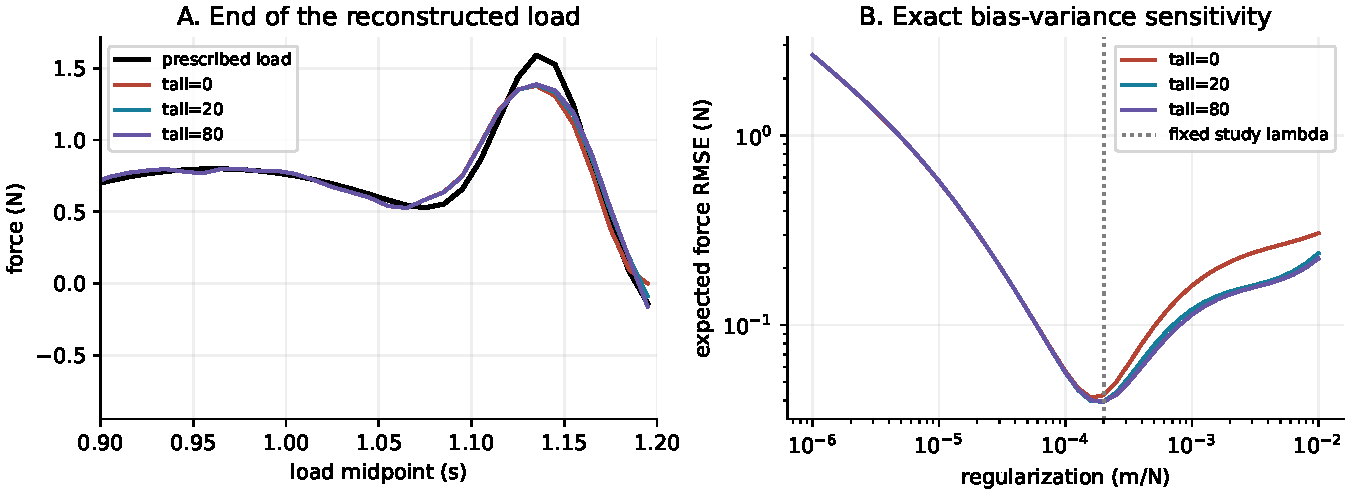
\includegraphics[width=\linewidth]{../examples/results/window-study.pdf}
\caption{Project-generated results. Left: one noisy reconstruction near the
load endpoint. Right: analytical expected RMSE over independent sensor noise,
conditional on the specified force and model. The vertical line marks the
fixed regularization used in Table~\ref{tab:risk}.}
\label{fig:study}
\end{figure}

\textbf{Discrete validation.} The largest coefficient discrepancy between
LSQR and the SVD ridge reference across the four windows is
$3.90\times10^{-9}$ N. LSQR terminates in 83--95 iterations in the recorded
local run; iteration counts can vary with platform rounding. A unit constant
force agrees with the analytical damped step response to
$1.48\times10^{-17}$ m maximum absolute error. These test the finite held-load
model and its inversion, not the fidelity of a physical experiment.

\newpage
\section{Continuum approximation, discussion, and limitations}
To separate propagation accuracy from forcing approximation, a second
experiment drives Equation~\eqref{eq:mechanics} with the smooth load
$f(t)=\sin(7t)$ N over $0\leq t\leq1.2$ s. A DOP853 reference uses relative
tolerance $2\times10^{-12}$ and absolute tolerance $2\times10^{-14}$.
Midpoint samples of this load are held constant in each interval and
propagated by Equation~\eqref{eq:exponential}. Maximum displacement errors
at the common sample points are listed below.

\begin{center}
\begin{tabular}{rrr}
\toprule
$\Delta t$ (s) & Maximum displacement error (m) & Previous/current error\\
\midrule
0.040 & $1.52331\times10^{-4}$ & ---\\
0.020 & $3.81391\times10^{-5}$ & 3.994\\
0.010 & $9.53830\times10^{-6}$ & 3.998\\
0.005 & $2.38690\times10^{-6}$ & 3.996\\
\bottomrule
\end{tabular}
\end{center}
This experiment exhibits approximately second-order sample-point
displacement convergence for a smooth input. It does not show second-order
pointwise force convergence: the held function is only a local constant
approximation. There is no spatial continuum mesh in this lumped model.
The exact held-load step response, the smooth-input approximation error,
and uncertainty about actual mechanics are therefore separate questions.

The tail is useful because late loads can influence subsequent state
evolution. Nevertheless, all post-load displacement samples depend on the
two-dimensional terminal state. They cannot supply an unlimited number of
independent load-history directions. A large terminal column norm is only
an isolated-load sensitivity measure: neighboring columns remain correlated.
It cannot by itself quantify identifiability when all forces are unknown.

The zero-tail result is especially cautionary. Ridge returns zero for the
unseen coefficient because that minimizes the penalty, not because the
measurements support a zero force. With longer tails, regularization continues
to trade noise amplification against bias, as the sweep shows. A data-driven
choice of $\lambda$, correlated-noise whitening, or a smoothness prior would
define different estimators and require separate validation.

\textbf{Limits of the evidence.} All data are synthetic, with one oscillator,
one load history, and a known unloaded tail. No experiment validates mass,
damping, stiffness, initial conditions, sensor dynamics, or the assumed noise.
Unmodeled tail forces can invalidate the inverse problem. Nonlinear response,
multiple unknown inputs, distributed mechanics, positivity constraints, and
automatic regularization selection are outside scope. Dense SVD and exact
risk evaluation are small-problem diagnostics; production matvecs remain
matrix-free. Linear complexity follows from the recurrences, but no measured
runtime advantage or large-scale throughput is claimed.

\section{Conclusion}
Observation timing creates an exact terminal-force nullspace in a finite
displacement record. An unloaded tail can reduce the endpoint error, but
one additional sample need not help a particular regularized estimate.
Independent discrete checks, explicit bias--variance accounting, and a
separate continuum-input experiment make these effects distinguishable.
The supplied implementation and recorded outputs permit this limited
synthetic conclusion to be reproduced without private source material.

\begin{thebibliography}{9}\small
\bibitem{paige} C.~C. Paige and M.~A. Saunders, ``LSQR: An algorithm for sparse
linear equations and sparse least squares,'' \emph{ACM Trans. Math. Softw.},
8(1), 43--71, 1982. Public software and reference:
\href{https://web.stanford.edu/group/SOL/software/lsqr/}{Stanford SOL: LSQR}.
\bibitem{scipyZOH} SciPy developers, \texttt{cont2discrete}: continuous-to-discrete
state-space conversion, API documentation. Accessed 13 October 2026.
\href{https://docs.scipy.org/doc/scipy/reference/generated/scipy.signal.cont2discrete.html}{SciPy signal documentation}.
\bibitem{scipyLSQR} SciPy developers, \texttt{lsqr}: damped least-squares solver,
API documentation. Accessed 13 October 2026.
\href{https://docs.scipy.org/doc/scipy/reference/generated/scipy.sparse.linalg.lsqr.html}{SciPy sparse linear algebra documentation}.
\end{thebibliography}
\end{document}
